% !TEX root = ../main.tex
% 本文件由 build-tex.sh 从 16-DSP指南-第16章中译.md 生成，改内容请改 md 后重新生成

\chapter{加窗 sinc 滤波器}\label{ch-16}

加窗 sinc 滤波器(windowed-sinc
filter)用来把一个频带与另一个频带分开。它们非常稳定，很少出意外，而且性能可以推到惊人的高度。这些出色的频域特性，是以时域表现很差为代价换来的，包括阶跃响应中过大的振铃(ripple)和过冲(overshoot)。用标准卷积实现时，加窗
sinc 滤波器很容易编程，但执行很慢。第 18 章会说明怎样用 FFT
大幅提高这类滤波器的计算速度。

\section{加窗 sinc 的思路}

图 16-1 说明了加窗 sinc 滤波器背后的想法。(a)
是理想低通滤波器的频率响应：低于截止频率 \(f_C\) 的所有频率都以幅度 1
通过，高于它的所有频率都被挡住。通带(passband)完全平坦，阻带(stopband)的衰减无穷大，两者之间的过渡无限窄。

对这个理想频率响应做逆傅里叶变换，就得到 (b)
所示的理想滤波器核（冲激响应）。前面讨论过（见第 11 章公式
11-4），这条曲线的一般形式是 \(\sin(x)/x\)，叫做 sinc 函数，表达式为：

\[h[i] = \frac{\sin(2\pi f_C\, i)}{i\pi}\]

把输入信号与这个滤波器核卷积，就是一个完美的低通滤波器。问题在于，sinc
函数一直延伸到负无穷和正无穷，幅度不会降到零。这种无限长度对数学不成问题，对计算机却是致命的。

为了绕开这个问题，我们对 (b) 中的 sinc 函数做两处修改，得到 (c)
所示的波形。第一，把它截断成 M+1 个点，围绕主瓣(main
lobe)对称地选取，其中 M 是偶数。这 M+1
个点以外的所有采样都设为零，或者干脆不管。第二，把整个序列向右平移，让它从
0 跑到
M。这样滤波器核只用正下标就能表示。虽然很多编程语言允许负下标，但用起来很麻烦。滤波器核平移
M/2 的唯一影响，是输出信号也平移同样的量。

由于修改后的滤波器核只是理想滤波器核的近似，它的频率响应不会是理想的。要知道实际得到的频率响应，可以对
(c) 中的信号做傅里叶变换，得到 (d)
中的曲线。一团糟！通带里有过大的波纹，阻带衰减很差（回想第 11
章讨论的吉布斯效应(Gibbs effect)）。这些问题源于截断后的 sinc
函数两端的突然间断。增加滤波器核的长度并不能减轻这些问题：不管 M
取多大，这个间断都很显著。

幸好有一个简单的办法能改善这种状况。(e)
是一条平滑渐收的曲线，叫做布莱克曼窗(Blackman window)。把截断的 sinc (c)
乘以布莱克曼窗 (e)，得到 (f) 所示的加窗 sinc
滤波器核。目的是让截断处不那么突兀，从而改善频率响应。(g)
显示了这一改善：通带现在是平的，阻带衰减好到在这张图上都看不出来。

可用的窗(window)有好几种，大多以 1950
年代最早提出它们的人命名。值得用的只有两种：汉明窗(Hamming
window)和布莱克曼窗。它们的表达式是：

\textbf{公式 16-1}　汉明窗。这些窗的 i 从 0 跑到 M，共 M+1 个点。

\[w[i] = 0.54 - 0.46\cos(2\pi i/M)\]

\textbf{公式 16-2}　布莱克曼窗。

\[w[i] = 0.42 - 0.5\cos(2\pi i/M) + 0.08\cos(4\pi i/M)\]

\begin{figure}[htbp]
\centering
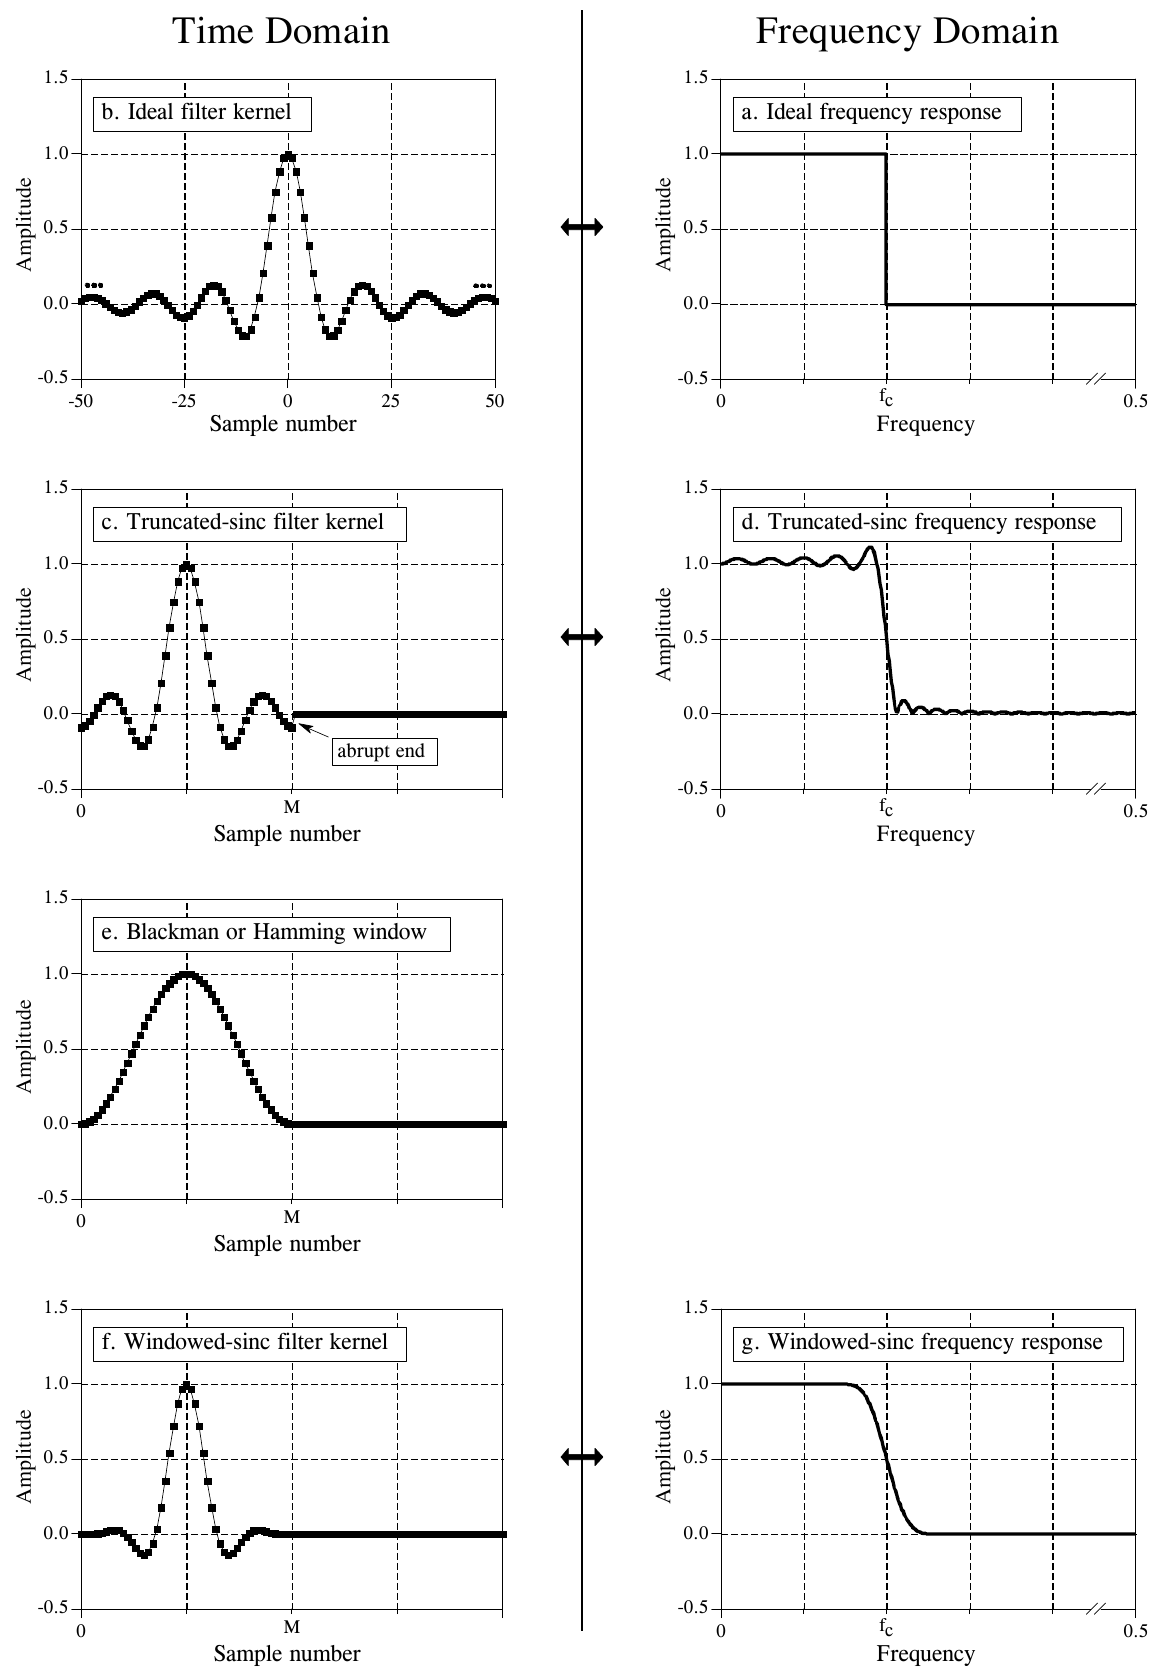
\includegraphics[width=0.958\linewidth,height=0.8\textheight,keepaspectratio]{assets/ch16/fig16-01.png}
\caption*{\textbf{图 16-1　加窗 sinc 滤波器核的推导。} (a)
是理想低通滤波器的频率响应，(b) 是对应的滤波器核，即 sinc 函数。由于
sinc 无限长，要在计算机里使用就必须截断，如 (c)
所示。然而，截断给频率响应带来了不希望有的变化 (d)。解决办法是把截断的
sinc 乘以一个平滑的窗 (e)，得到加窗 sinc 滤波器核 (f)。加窗 sinc
的频率响应 (g) 平滑而规矩。这些图没有按比例绘制。 （Time Domain =
时域，Frequency Domain = 频域；a. Ideal frequency response =
理想频率响应，b. Ideal filter kernel = 理想滤波器核，c.~Truncated-sinc
filter kernel = 截断 sinc 滤波器核，d.~Truncated-sinc frequency response
= 截断 sinc 的频率响应，e. Blackman or Hamming window =
布莱克曼窗或汉明窗，f.~Windowed-sinc filter kernel = 加窗 sinc
滤波器核，g. Windowed-sinc frequency response = 加窗 sinc
的频率响应；abrupt end = 突然截断的端点。Amplitude = 幅度，Sample number
= 采样序号，Frequency = 频率。原书这张图排在单独一页，图注写作 ``facing
page''（见对页）。）}
\end{figure}

图 16-2a 画出了 M = 50（即曲线共 51
个点）时这两种窗的形状。该用哪一种？这是参数之间的权衡。如图 16-2b
所示，汉明窗的滚降(roll-off)比布莱克曼窗快约 20\%。然而，(c)
表明布莱克曼窗的阻带衰减更好。确切地说，布莱克曼窗的阻带衰减是 −74
dB（约 0.02\%），而汉明窗只有 −53 dB（约
0.2\%）。虽然在这些图里看不出来，布莱克曼窗的通带波纹只有约
0.02\%，而汉明窗一般是
0.2\%。总的来说，布莱克曼窗应当是你的首选：滚降慢一点比阻带衰减差更容易应付。

\begin{figure}[htbp]
\centering
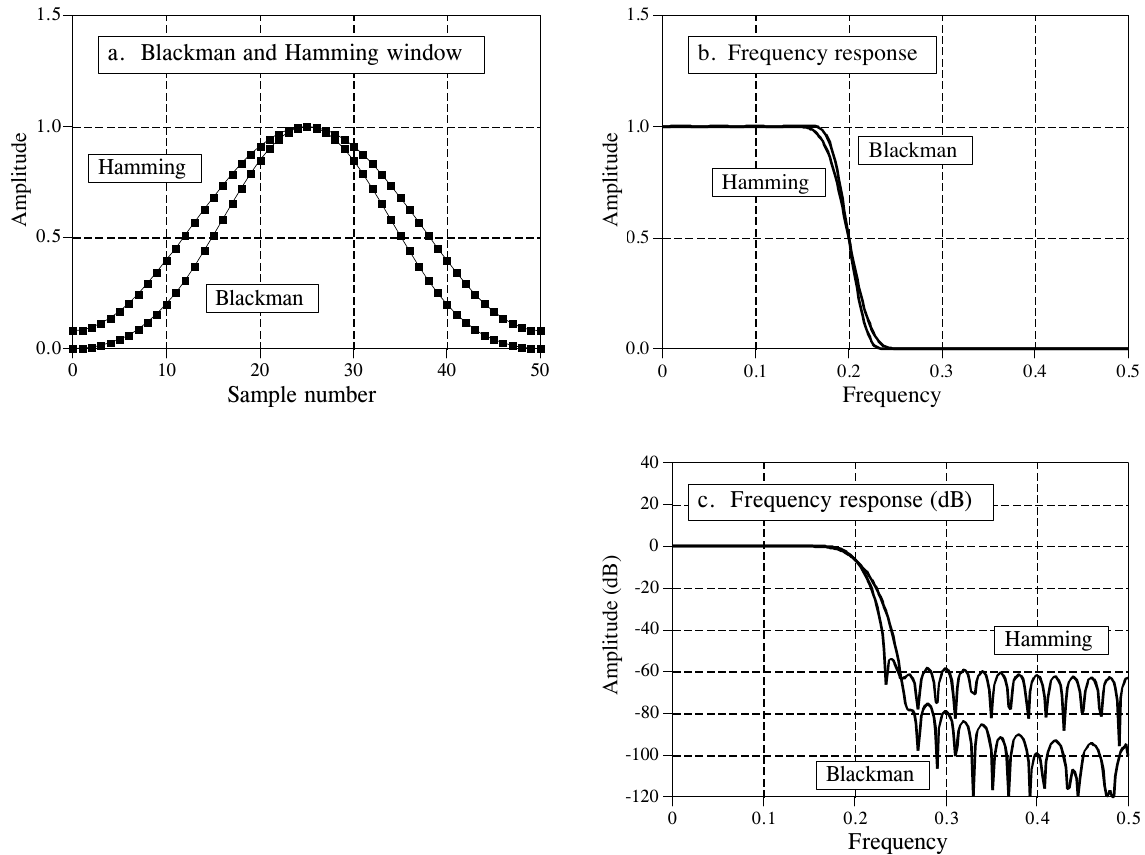
\includegraphics[width=0.954\linewidth,height=0.8\textheight,keepaspectratio]{assets/ch16/fig16-02.png}
\caption*{\textbf{图 16-2　布莱克曼窗和汉明窗的特性。} (a)
是这两种窗的形状，由公式 16-1 和 16-2 给出。如 (b)
所示，汉明窗的滚降比布莱克曼窗快约
20\%。然而，布莱克曼窗的阻带衰减更好（布莱克曼：0.02\%，汉明：0.2\%），通带波纹也更低（布莱克曼：0.02\%，汉明：0.2\%）。
（a. Blackman and Hamming window = 布莱克曼窗与汉明窗，b. Frequency
response = 频率响应，c.~Frequency response (dB) =
频率响应（分贝）；Hamming = 汉明，Blackman = 布莱克曼。Amplitude =
幅度，Amplitude (dB) = 幅度（分贝），Sample number = 采样序号，Frequency
= 频率。原书英文图注排在 (c) 左侧，裁图时已擦掉，译文见上。）}
\end{figure}

你可能还会听说别的窗，不过它们都比不上布莱克曼窗和汉明窗。巴特利特窗(Bartlett
window)是一个三角形，用直线做渐收。汉宁窗(Hanning
window)也叫升余弦窗(raised cosine window)，表达式是
\(w[i] = 0.5 - 0.5\cos(2\pi i/M)\)。这两种窗的滚降速度和汉明窗差不多，但阻带衰减更差（巴特利特：−25
dB，即 5.6\%；汉宁：−44 dB，即 0.63\%）。你也可能听说矩形窗(rectangular
window)。它等于不加窗，只是把尾部截掉（就像图 16-1c
那样）。它的滚降比布莱克曼窗快约 2.5 倍，但阻带衰减只有 −21
dB（8.9\%）。

\section{设计滤波器}

设计一个加窗 sinc 滤波器要选两个参数：截止频率 \(f_C\) 和滤波器核的长度
M。截止频率用采样率的分数表示，因此必须在 0 到 0.5 之间。M
的取值按下面的近似式决定滚降：

\textbf{公式 16-3}　滤波器长度与滚降的关系。滤波器核的长度 M
决定滤波器的过渡带宽 BW。这只是一个近似，因为滚降还取决于所用的窗。

\[M \approx \frac{4}{BW}\]

其中 BW 是过渡带(transition band)的宽度，从曲线刚刚离开 1
的地方量到它几乎降到 0 的地方（比如曲线的 99\% 到
1\%）。过渡带宽也用采样频率的分数表示，必须在 0 到 0.5 之间。图 16-3a
是使用这个近似式的一个例子。图中三条曲线由 M = 20、40 和 200
的滤波器核得到。由公式 16-3，过渡带宽分别是 BW = 0.2、0.1 和 0.02。(b)
表明频率响应的形状不随所选的截止频率变化。

\begin{figure}[htbp]
\centering
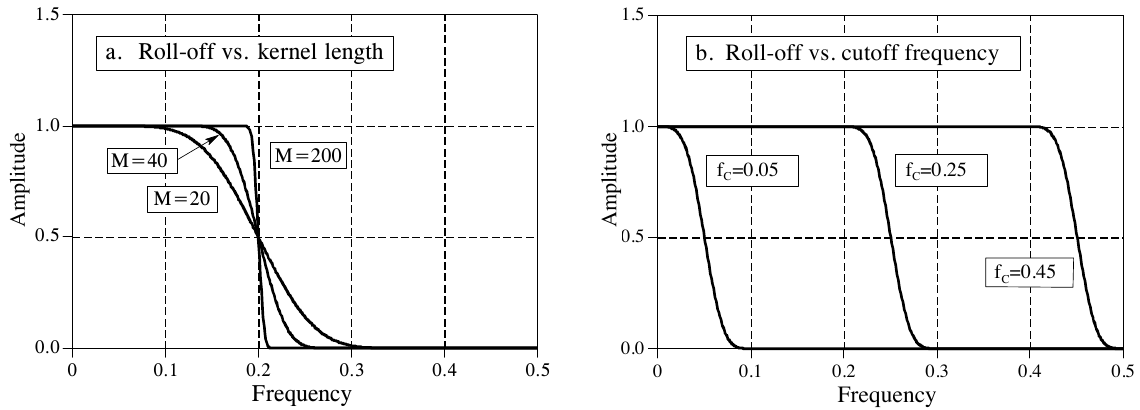
\includegraphics[width=0.950\linewidth,height=0.8\textheight,keepaspectratio]{assets/ch16/fig16-03.png}
\caption*{\textbf{图 16-3　加窗 sinc 滤波器的长度与滚降。} 如 (a) 所示，M = 20、40
和 200 时，过渡带宽分别是采样率的 BW = 0.2、0.1 和 0.02。如 (b)
所示，截止频率不同时，频率响应的形状不变。(b) 中 M = 60。 （a. Roll-off
vs.~kernel length = 滚降与核长度，b. Roll-off vs.~cutoff frequency =
滚降与截止频率。Amplitude = 幅度，Frequency = 频率。）}
\end{figure}

由于卷积所需的时间与信号长度成正比，公式 16-3 体现的是计算时间（取决于
M）与滤波器陡峭程度（BW
的值）之间的权衡。例如，布莱克曼窗（与汉明窗相比）慢 20\%
的滚降，可以用长 20\%
的滤波器核来弥补。换句话说，可以说布莱克曼窗比滚降相当的汉明窗执行起来慢
20\%。这一点很重要，因为加窗 sinc 滤波器的执行速度本来就慢得要命。

同样如图 16-3b 所示，加窗 sinc
滤波器的截止频率是在幅度一半的地方测量的。为什么用
0.5，而不用模拟电子学和其他数字滤波器中标准的 0.707（−3
dB）？这是因为加窗 sinc
的频率响应在通带和阻带之间是对称的。例如，汉明窗的通带波纹是
0.2\%，阻带衰减（即阻带中的波纹）也同样是
0.2\%。其他滤波器没有这种对称性，因此用半幅点标记截止频率对它们没有好处。本章后面会看到，这种对称性使加窗
sinc 非常适合做频谱反转(spectral inversion)。

选好 \(f_C\) 和 M 之后，滤波器核按下式计算：

\textbf{公式 16-4}　加窗 sinc 滤波器核。截止频率 \(f_C\)
用采样率的分数表示，取值在 0 到 0.5 之间。滤波器核的长度由 M 决定，M
必须是偶数。采样序号 i 是从 0 到 M 的整数，滤波器核共 M+1 个点。常数 K
的选取使零频率处的增益为 1。为避免除零错误，在 i = M/2 处取
\(h[i] = 2\pi f_C K\)。

\[h[i] = K\,\frac{\sin\!\big(2\pi f_C\,(i - M/2)\big)}{i - M/2}\left[0.42 - 0.5\cos\!\left(\frac{2\pi i}{M}\right) + 0.08\cos\!\left(\frac{4\pi i}{M}\right)\right]\]

别被这个式子吓住！根据前面的讨论，你应该能认出其中的三个部分：sinc
函数、M/2 的平移和布莱克曼窗。要让滤波器在直流处的增益为 1，常数 K
必须选得使所有采样之和等于 1。实际做法是：算滤波器核时先不管
K，算完再把所有采样按需要归一化。表 16-1 的程序展示了怎样做。还要注意
sinc 中心 i = M/2 处的计算是怎么处理的，那里会出现除以零。

这个式子虽然长，用起来却很简单：把它敲进程序就可以不管了，让计算机去算。如果你发现自己在手算这个式子，那你一定是做错了什么。

具体说一下公式 16-4
描述的滤波器核在计算机数组里放在什么位置。举个例子，取 M = 100。记住，M
必须是偶数。滤波器核的第一个点在数组位置 0，最后一个点在数组位置
100。这意味着整个信号长 101 个点。对称中心在第 50 点，即 M/2。第 50
点左边的 50 个点与右边的 50 个点对称：第 0 点与第 100 点的值相同，第 49
点与第 51 点相同。如果你一定要让滤波器核有特定数量的采样（比如为了用
FFT），只要在一端或另一端补零即可。例如 M = 100 时，可以把第 101 到 127
个采样设为零，得到一个 128 点长的滤波器核。

\begin{figure}[htbp]
\centering
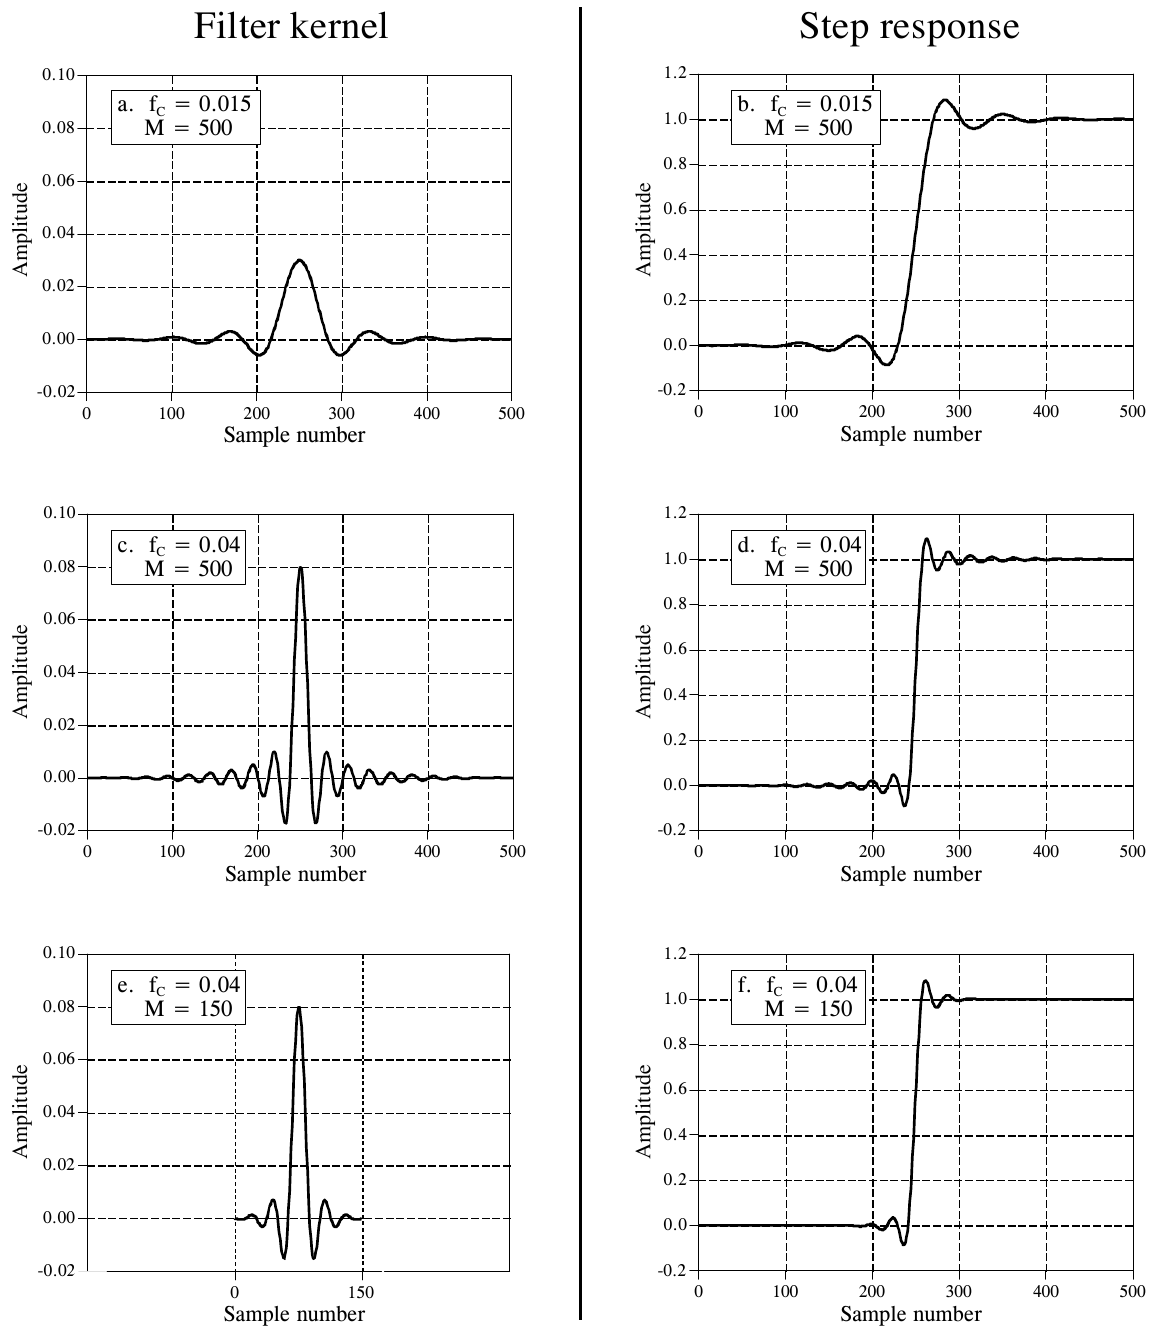
\includegraphics[width=0.958\linewidth,height=0.8\textheight,keepaspectratio]{assets/ch16/fig16-04.png}
\caption*{\textbf{图 16-4　滤波器核示例及对应的阶跃响应。}
正弦振荡的频率大约等于截止频率 \(f_C\)，而 M 决定核的长度。 （Filter
kernel = 滤波器核，Step response = 阶跃响应。Amplitude = 幅度，Sample
number = 采样序号。(e) 的横轴在原书 PDF 中抽取时显示为 ``−175 0
150175''，图上实际只标了 0 和 150。）}
\end{figure}

图 16-4 给出了加窗 sinc 滤波器核的例子，以及它们对应的阶跃响应(step
response)。滤波器核开头和结尾的采样非常小，在图上甚至看不出来。别误以为它们不重要！这些采样的值也许很小，但它们合起来对滤波器的性能有很大影响。这也是加窗
sinc
滤波器通常用浮点数实现的原因：整数通常没有足够的动态范围，装不下滤波器核里大小悬殊的数值。加窗
sinc
滤波器在时域表现如何？很糟糕！阶跃响应有过冲和振铃；对于信息编码在时域里的信号，这不是该用的滤波器。

\section{加窗 sinc 滤波器的例子}

脑电图（electroencephalogram，EEG）是对大脑电活动的测量。它可以通过贴在头皮表面的电极测到，是毫伏级的信号。大脑中的每个神经细胞都会产生微小的电脉冲。EEG
是大量这种电脉冲以（但愿是）协调的方式产生后的综合结果。虽然人们对思维与这种电协调之间的关系知之甚少，但
EEG 中的不同频率可以和特定的精神状态对应起来。如果你闭上眼睛放松，EEG
的主要模式会是一个约 7 到 12 赫兹之间的缓慢振荡。这个波形叫做 α
节律(alpha rhythm)，与满足和注意力下降有关。睁开眼睛四处张望，EEG 会变成
β 节律(beta rhythm)，频率约在 17 到 20
赫兹之间。在儿童身上、不同深度的睡眠中，以及癫痫等各种脑部疾病中，还能看到其他频率和波形。

在这个例子中，我们假设 EEG 信号已经由模拟电路放大，然后以每秒 100
个采样的采样率数字化。采集 50 秒的数据，得到一个 5000
点的信号。我们的目标是把 α 节律和 β
节律分开。为此，我们设计一个截止频率为 14 赫兹（即采样率的
0.14）的数字低通滤波器。过渡带宽定为 4 赫兹，即采样率的 0.04。由公式
16-3，滤波器核需要约 101 个点长，我们随意选用汉明窗。表 16-1
的程序展示了怎样实现这个滤波器。对滤波器核做傅里叶变换得到的频率响应，如图
16-5 所示。

\begin{figure}[htbp]
\centering
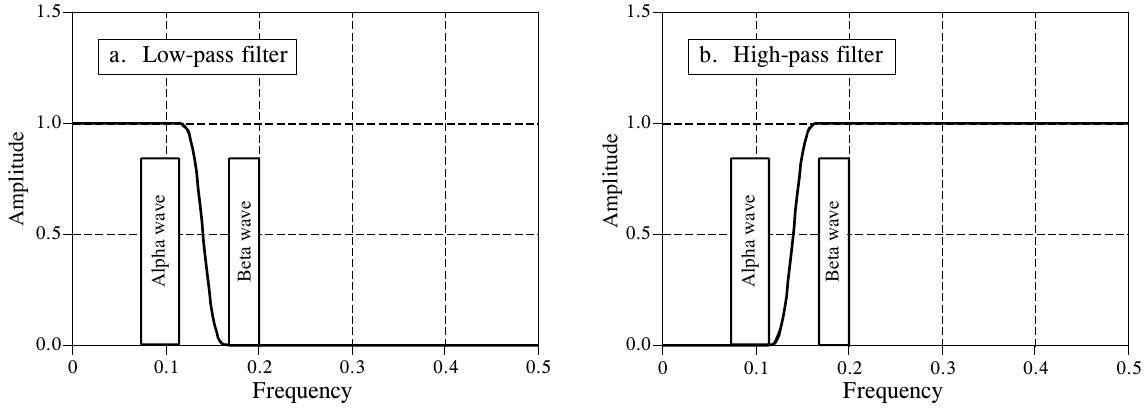
\includegraphics[width=0.954\linewidth,height=0.8\textheight,keepaspectratio]{assets/ch16/fig16-05.png}
\caption*{\textbf{图 16-5　加窗 sinc 滤波器的例子。} 用 M = 100
的低通和高通滤波器把 EEG 中的 α 节律和 β
节律分开。实现低通滤波器的程序见表
16-1。高通滤波器的程序与之相同，只是对低通滤波器核做了频谱反转。 （a.
Low-pass filter = 低通滤波器，b. High-pass filter = 高通滤波器；Alpha
wave = α 波，Beta wave = β 波。Amplitude = 幅度，Frequency = 频率。）}
\end{figure}

\textbf{表 16-1}（注释已译成中文）

\begin{Shaded}
\begin{Highlighting}[]
\NormalTok{100 \textquotesingle{}LOW{-}PASS WINDOWED{-}SINC FILTER}
\NormalTok{110 \textquotesingle{}本程序用 101 点的加窗 sinc 滤波器对 5000 个采样滤波，}
\NormalTok{120 \textquotesingle{}得到 4900 个滤波后的数据。}
\NormalTok{130 \textquotesingle{}}
\NormalTok{140 DIM X[4999]                       \textquotesingle{}X[ ] 存放输入信号}
\NormalTok{150 DIM Y[4999]                       \textquotesingle{}Y[ ] 存放输出信号}
\NormalTok{160 DIM H[100]                        \textquotesingle{}H[ ] 存放滤波器核}
\NormalTok{170 \textquotesingle{}}
\NormalTok{180 PI = 3.14159265}
\NormalTok{190 FC = .14                          \textquotesingle{}设定截止频率（0 到 0.5 之间）}
\NormalTok{200 M\% = 100                          \textquotesingle{}设定滤波器长度（101 点）}
\NormalTok{210 \textquotesingle{}}
\NormalTok{220 GOSUB XXXX                        \textquotesingle{}虚构的子程序，载入 X[ ]}
\NormalTok{230 \textquotesingle{}}
\NormalTok{240 \textquotesingle{}                                 \textquotesingle{}按公式 16{-}4 计算低通滤波器核}
\NormalTok{250 FOR I\% = 0 TO 100}
\NormalTok{260 IF (I\%{-}M\%/2) = 0 THEN H[I\%] = 2*PI*FC}
\NormalTok{270 IF (I\%{-}M\%/2) \textless{}\textgreater{} 0 THEN H[I\%] = SIN(2*PI*FC * (I\%{-}M\%/2)) / (I\%{-}M\%/2)}
\NormalTok{280 H[I\%] = H[I\%] * (0.54 {-} 0.46*COS(2*PI*I\%/M\%) )}
\NormalTok{290 NEXT I\%}
\NormalTok{300 \textquotesingle{}}
\NormalTok{310 SUM = 0                           \textquotesingle{}把低通滤波器核归一化，}
\NormalTok{320 FOR I\% = 0 TO 100                 \textquotesingle{}使直流增益为 1}
\NormalTok{330 SUM = SUM + H[I\%]}
\NormalTok{340 NEXT I\%}
\NormalTok{350 \textquotesingle{}}
\NormalTok{360 FOR I\% = 0 TO 100}
\NormalTok{370 H[I\%] = H[I\%] / SUM}
\NormalTok{380 NEXT I\%}
\NormalTok{390 \textquotesingle{}}
\NormalTok{400 FOR J\% = 100 TO 4999              \textquotesingle{}输入信号与滤波器核卷积}
\NormalTok{410 Y[J\%] = 0}
\NormalTok{420 FOR I\% = 0 TO 100}
\NormalTok{430     Y[J\%] = Y[J\%] + X[J\%{-}I\%] * H[I\%]}
\NormalTok{440 NEXT I\%}
\NormalTok{450 NEXT J\%}
\NormalTok{460 \textquotesingle{}}
\NormalTok{470 END}
\end{Highlighting}
\end{Shaded}

\textbf{C 实现}（完整可编译版本见
\texttt{c/table16-1\_lowpass\_windowed\_sinc.c}，其中用 10 Hz 的 α
正弦加 18 Hz 的 β 正弦造了一段假 EEG，并直接计算滤波器核的频率响应）：

\begin{Shaded}
\begin{Highlighting}[]
\CommentTok{/* 第 240～380 行：按公式 16{-}4 算低通滤波器核，再归一化到直流增益为 1 */}
\DataTypeTok{static} \DataTypeTok{void}\NormalTok{ lowpass\_kernel}\OperatorTok{(}\DataTypeTok{double}\NormalTok{ fc}\OperatorTok{,} \DataTypeTok{double} \OperatorTok{*}\NormalTok{h}\OperatorTok{)}
\OperatorTok{\{}
    \ControlFlowTok{for} \OperatorTok{(}\DataTypeTok{int}\NormalTok{ i }\OperatorTok{=} \DecValTok{0}\OperatorTok{;}\NormalTok{ i }\OperatorTok{\textless{}=}\NormalTok{ M}\OperatorTok{;}\NormalTok{ i}\OperatorTok{++)} \OperatorTok{\{}          \CommentTok{/* 250 */}
        \ControlFlowTok{if} \OperatorTok{(}\NormalTok{i }\OperatorTok{{-}}\NormalTok{ M }\OperatorTok{/} \DecValTok{2} \OperatorTok{==} \DecValTok{0}\OperatorTok{)}\NormalTok{ h}\OperatorTok{[}\NormalTok{i}\OperatorTok{]} \OperatorTok{=} \FloatTok{2.0} \OperatorTok{*}\NormalTok{ PI }\OperatorTok{*}\NormalTok{ fc}\OperatorTok{;}                             \CommentTok{/* 260：sinc 中心，避免除零 */}
        \ControlFlowTok{else}\NormalTok{                h}\OperatorTok{[}\NormalTok{i}\OperatorTok{]} \OperatorTok{=}\NormalTok{ sin}\OperatorTok{(}\FloatTok{2.0} \OperatorTok{*}\NormalTok{ PI }\OperatorTok{*}\NormalTok{ fc }\OperatorTok{*} \OperatorTok{(}\NormalTok{i }\OperatorTok{{-}}\NormalTok{ M }\OperatorTok{/} \DecValTok{2}\OperatorTok{))} \OperatorTok{/} \OperatorTok{(}\NormalTok{i }\OperatorTok{{-}}\NormalTok{ M }\OperatorTok{/} \DecValTok{2}\OperatorTok{);} \CommentTok{/* 270 */}
\NormalTok{        h}\OperatorTok{[}\NormalTok{i}\OperatorTok{]} \OperatorTok{*=} \FloatTok{0.54} \OperatorTok{{-}} \FloatTok{0.46} \OperatorTok{*}\NormalTok{ cos}\OperatorTok{(}\FloatTok{2.0} \OperatorTok{*}\NormalTok{ PI }\OperatorTok{*}\NormalTok{ i }\OperatorTok{/}\NormalTok{ M}\OperatorTok{);}                          \CommentTok{/* 280：乘汉明窗（公式 16{-}1） */}
    \OperatorTok{\}}

    \DataTypeTok{double}\NormalTok{ sum }\OperatorTok{=} \FloatTok{0.0}\OperatorTok{;}                       \CommentTok{/* 310～340：求和 */}
    \ControlFlowTok{for} \OperatorTok{(}\DataTypeTok{int}\NormalTok{ i }\OperatorTok{=} \DecValTok{0}\OperatorTok{;}\NormalTok{ i }\OperatorTok{\textless{}=}\NormalTok{ M}\OperatorTok{;}\NormalTok{ i}\OperatorTok{++)}\NormalTok{ sum }\OperatorTok{+=}\NormalTok{ h}\OperatorTok{[}\NormalTok{i}\OperatorTok{];}
    \ControlFlowTok{for} \OperatorTok{(}\DataTypeTok{int}\NormalTok{ i }\OperatorTok{=} \DecValTok{0}\OperatorTok{;}\NormalTok{ i }\OperatorTok{\textless{}=}\NormalTok{ M}\OperatorTok{;}\NormalTok{ i}\OperatorTok{++)}\NormalTok{ h}\OperatorTok{[}\NormalTok{i}\OperatorTok{]} \OperatorTok{/=}\NormalTok{ sum}\OperatorTok{;}   \CommentTok{/* 360～380：归一化，直流增益为 1 */}
\OperatorTok{\}}

\CommentTok{/* 第 400～450 行：卷积，只算滤波器核完全浸没在输入里的输出点 */}
\DataTypeTok{static} \DataTypeTok{void}\NormalTok{ convolve}\OperatorTok{(}\DataTypeTok{const} \DataTypeTok{double} \OperatorTok{*}\NormalTok{x}\OperatorTok{,} \DataTypeTok{const} \DataTypeTok{double} \OperatorTok{*}\NormalTok{h}\OperatorTok{,} \DataTypeTok{double} \OperatorTok{*}\NormalTok{y}\OperatorTok{)}
\OperatorTok{\{}
    \ControlFlowTok{for} \OperatorTok{(}\DataTypeTok{int}\NormalTok{ j }\OperatorTok{=}\NormalTok{ M}\OperatorTok{;}\NormalTok{ j }\OperatorTok{\textless{}}\NormalTok{ NX}\OperatorTok{;}\NormalTok{ j}\OperatorTok{++)} \OperatorTok{\{}          \CommentTok{/* 400：FOR J\% = 100 TO 4999 */}
\NormalTok{        y}\OperatorTok{[}\NormalTok{j}\OperatorTok{]} \OperatorTok{=} \FloatTok{0.0}\OperatorTok{;}                         \CommentTok{/* 410 */}
        \ControlFlowTok{for} \OperatorTok{(}\DataTypeTok{int}\NormalTok{ i }\OperatorTok{=} \DecValTok{0}\OperatorTok{;}\NormalTok{ i }\OperatorTok{\textless{}=}\NormalTok{ M}\OperatorTok{;}\NormalTok{ i}\OperatorTok{++)}        \CommentTok{/* 420 */}
\NormalTok{            y}\OperatorTok{[}\NormalTok{j}\OperatorTok{]} \OperatorTok{+=}\NormalTok{ x}\OperatorTok{[}\NormalTok{j }\OperatorTok{{-}}\NormalTok{ i}\OperatorTok{]} \OperatorTok{*}\NormalTok{ h}\OperatorTok{[}\NormalTok{i}\OperatorTok{];}        \CommentTok{/* 430 */}
    \OperatorTok{\}}
\OperatorTok{\}}
\end{Highlighting}
\end{Shaded}

运行结果： - 101 个系数之和为 1.000000000000（直流增益为 1）；h{[}0{]}
与 h{[}100{]}、h{[}49{]} 与 h{[}51{]} 完全相等，左右对称。 -
频率响应：10 Hz 处 0.9995，截止频率 14 Hz（0.14）处
0.5003，正好是半幅点；f \dspsym{≥} 0.18 的阻带最大残留约 −59 dB，16 Hz
处约 −53 dB，与正文说的汉明窗阻带衰减 −53 dB 吻合。 - 滤波后：10 Hz 的 α
分量剩 0.9995，18 Hz 的 β 分量只剩 0.0011，两个节律被分开了。

第二个例子，我们设计一个带通滤波器(band-pass
filter)，用来从音频信号中分离出一个信令音，比如按下电话按键时发出的声音。假设信号以
10 kHz 数字化，目标是分离出以 2 kHz 为中心、宽 80
赫兹的频带。用采样率表示，我们要挡掉所有低于 0.196 和高于 0.204
的频率（分别对应 1960 赫兹和 2040 赫兹）。为了得到 50 赫兹（采样率的
0.005）的过渡带宽，我们让滤波器核长 801 个点，并使用布莱克曼窗。表 16-2
是计算这个滤波器核的程序，图 16-6
是它的频率响应。设计分几步。第一，设计两个低通滤波器，一个截止在
0.196，另一个截止在
0.204。然后对第二个滤波器做频谱反转，把它变成高通滤波器（见第 14 章图
14-6）。接着把两个滤波器核相加，得到一个带阻滤波器（band-reject
filter，见图 14-8）。最后再做一次频谱反转，把它变成我们要的带通滤波器。

\begin{figure}[htbp]
\centering
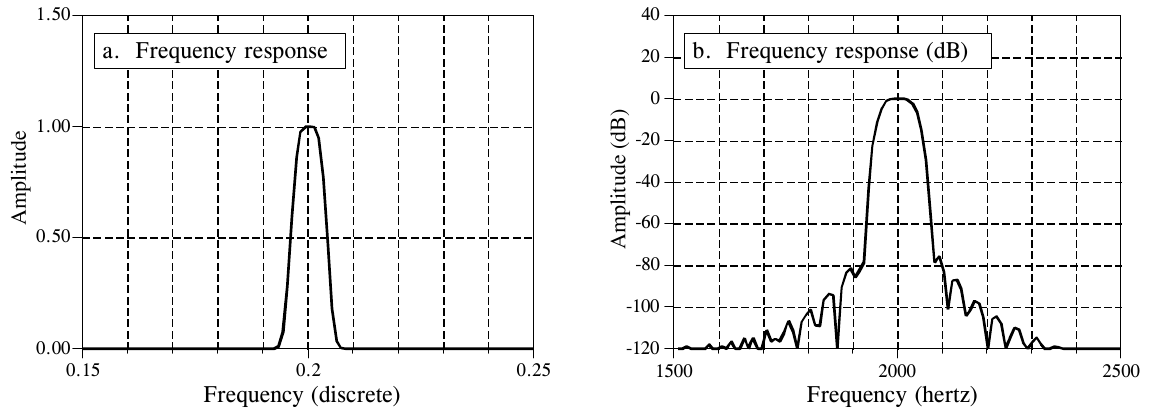
\includegraphics[width=0.958\linewidth,height=0.8\textheight,keepaspectratio]{assets/ch16/fig16-06.png}
\caption*{\textbf{图 16-6　加窗 sinc 带通滤波器的例子。} 这个滤波器是按 10 kHz
采样率设计的。对应到模拟信号，通带中心频率在 2 kHz，通带宽 80
赫兹，过渡带宽 50 赫兹。加窗 sinc 的滤波器核用了 801
个点来达到这样的滚降，并用布莱克曼窗获得良好的阻带衰减。(a)
是线性刻度的频率响应，(b) 是分贝刻度。(a)
的频率轴用采样频率的分数表示，(b) 则用数字化之前模拟信号的频率表示。
（a. Frequency response = 频率响应，b. Frequency response (dB) =
频率响应（分贝）；Frequency (discrete) = 频率（离散），Frequency (hertz)
= 频率（赫兹），Amplitude (dB) = 幅度（分贝）。(b) 纵轴 0
下面的刻度在原书图中显示为 ``20''，应为 −20。）}
\end{figure}

\textbf{表 16-2}（注释已译成中文）

\begin{Shaded}
\begin{Highlighting}[]
\NormalTok{100 \textquotesingle{}BAND{-}PASS WINDOWED{-}SINC FILTER}
\NormalTok{110 \textquotesingle{}本程序计算一个 801 点的带通滤波器核}
\NormalTok{120 \textquotesingle{}}
\NormalTok{130 DIM A[800]                      \textquotesingle{}A[ ] 是下截止频率的工作区}
\NormalTok{140 DIM B[800]                      \textquotesingle{}B[ ] 是上截止频率的工作区}
\NormalTok{150 DIM H[800]                      \textquotesingle{}H[ ] 存放最终的滤波器核}
\NormalTok{160 \textquotesingle{}}
\NormalTok{170 PI = 3.1415926}
\NormalTok{180 M\% = 800                        \textquotesingle{}设定滤波器核长度（801 点）}
\NormalTok{190 \textquotesingle{}}
\NormalTok{200 \textquotesingle{}                               \textquotesingle{}按公式 16{-}4 计算第一个低通滤波器核，}
\NormalTok{210 FC = 0.196                      \textquotesingle{}截止频率 0.196，存在 A[ ]}
\NormalTok{220 FOR I\% = 0 TO 800}
\NormalTok{230 IF (I\%{-}M\%/2) = 0 THEN A[I\%] = 2*PI*FC}
\NormalTok{240 IF (I\%{-}M\%/2) \textless{}\textgreater{} 0 THEN A[I\%] = SIN(2*PI*FC * (I\%{-}M\%/2)) / (I\%{-}M\%/2)}
\NormalTok{250 A[I\%] = A[I\%] * (0.42 {-} 0.5*COS(2*PI*I\%/M\%) + 0.08*COS(4*PI*I\%/M\%))}
\NormalTok{260 NEXT I\%}
\NormalTok{270 \textquotesingle{}}
\NormalTok{280 SUM = 0                         \textquotesingle{}把第一个低通滤波器核归一化，}
\NormalTok{290 FOR I\% = 0 TO 800               \textquotesingle{}使直流增益为 1}
\NormalTok{300 SUM = SUM + A[I\%]}
\NormalTok{310 NEXT I\%}
\NormalTok{320 \textquotesingle{}}
\NormalTok{330 FOR I\% = 0 TO 800}
\NormalTok{340 A[I\%] = A[I\%] / SUM}
\NormalTok{350 NEXT I\%}
\NormalTok{360 \textquotesingle{}                               \textquotesingle{}按公式 16{-}4 计算第二个低通滤波器核，}
\NormalTok{370 FC = 0.204                      \textquotesingle{}截止频率 0.204，存在 B[ ]}
\NormalTok{380 FOR I\% = 0 TO 800}
\NormalTok{390 IF (I\%{-}M\%/2) = 0 THEN B[I\%] = 2*PI*FC}
\NormalTok{400 IF (I\%{-}M\%/2) \textless{}\textgreater{} 0 THEN B[I\%] = SIN(2*PI*FC * (I\%{-}M\%/2)) / (I\%{-}M\%/2)}
\NormalTok{410 B[I\%] = B[I\%] * (0.42 {-} 0.5*COS(2*PI*I\%/M\%) + 0.08*COS(4*PI*I\%/M\%))}
\NormalTok{420 NEXT I\%}
\NormalTok{430 \textquotesingle{}}
\NormalTok{440 SUM = 0                         \textquotesingle{}把第二个低通滤波器核归一化，}
\NormalTok{450 FOR I\% = 0 TO 800               \textquotesingle{}使直流增益为 1}
\NormalTok{460 SUM = SUM + B[I\%]}
\NormalTok{470 NEXT I\%}
\NormalTok{480 \textquotesingle{}}
\NormalTok{490 FOR I\% = 0 TO 800}
\NormalTok{500 B[I\%] = B[I\%] / SUM}
\NormalTok{510 NEXT I\%}
\NormalTok{520 \textquotesingle{}}
\NormalTok{530 FOR I\% = 0 TO 800               \textquotesingle{}用频谱反转把 B[ ] 中的低通滤波器核}
\NormalTok{540 B[I\%] = {-} B[I\%]                 \textquotesingle{}变成高通滤波器核（如图 14{-}5）}
\NormalTok{550 NEXT I\%}
\NormalTok{560 B[400] = B[400] + 1}
\NormalTok{570 \textquotesingle{}}
\NormalTok{580 \textquotesingle{}}
\NormalTok{590 FOR I\% = 0 TO 800               \textquotesingle{}把 A[ ] 中的低通滤波器核与 B[ ] 中的高通}
\NormalTok{600 H[I\%] = A[I\%] + B[I\%]           \textquotesingle{}滤波器核相加，得到带阻滤波器核，}
\NormalTok{610 NEXT I\%                         \textquotesingle{}存在 H[ ] 中（如图 14{-}8）}
\NormalTok{620 \textquotesingle{}}
\NormalTok{630 FOR I\% = 0 TO 800               \textquotesingle{}用频谱反转把带阻滤波器核}
\NormalTok{640 H[I\%] = {-}H[I\%]                  \textquotesingle{}变成带通滤波器核}
\NormalTok{650 NEXT I\%}
\NormalTok{660 H[400] = H[400] + 1}
\NormalTok{670 \textquotesingle{}                               \textquotesingle{}带通滤波器核现在存放在 H[ ] 中}
\NormalTok{680 END}
\end{Highlighting}
\end{Shaded}

\begin{quote}
\textbf{译注：} 第 540 行注释说频谱反转''如图
14-5''，而正文讲同一步骤时引的是''第 14 章图
14-6''，两处图号不同，但都没错：第 14 章里图 14-5
是频谱反转的例子（滤波器核与频率响应），图 14-6
是频谱反转的框图，讲的是同一件事。
\end{quote}

\textbf{C 实现}（完整可编译版本见
\texttt{c/table16-2\_bandpass\_windowed\_sinc.c}，程序最后直接计算滤波器核的频率响应）：

\begin{Shaded}
\begin{Highlighting}[]
\CommentTok{/* 第 200～350 行（以及 360～510 行）：按公式 16{-}4 算低通核（布莱克曼窗），归一化到直流增益为 1 */}
\DataTypeTok{static} \DataTypeTok{void}\NormalTok{ lowpass\_kernel}\OperatorTok{(}\DataTypeTok{double}\NormalTok{ fc}\OperatorTok{,} \DataTypeTok{double} \OperatorTok{*}\NormalTok{a}\OperatorTok{)}
\OperatorTok{\{}
    \ControlFlowTok{for} \OperatorTok{(}\DataTypeTok{int}\NormalTok{ i }\OperatorTok{=} \DecValTok{0}\OperatorTok{;}\NormalTok{ i }\OperatorTok{\textless{}=}\NormalTok{ M}\OperatorTok{;}\NormalTok{ i}\OperatorTok{++)} \OperatorTok{\{}          \CommentTok{/* 220 */}
        \ControlFlowTok{if} \OperatorTok{(}\NormalTok{i }\OperatorTok{{-}}\NormalTok{ M }\OperatorTok{/} \DecValTok{2} \OperatorTok{==} \DecValTok{0}\OperatorTok{)}\NormalTok{ a}\OperatorTok{[}\NormalTok{i}\OperatorTok{]} \OperatorTok{=} \FloatTok{2.0} \OperatorTok{*}\NormalTok{ PI }\OperatorTok{*}\NormalTok{ fc}\OperatorTok{;}                             \CommentTok{/* 230 */}
        \ControlFlowTok{else}\NormalTok{                a}\OperatorTok{[}\NormalTok{i}\OperatorTok{]} \OperatorTok{=}\NormalTok{ sin}\OperatorTok{(}\FloatTok{2.0} \OperatorTok{*}\NormalTok{ PI }\OperatorTok{*}\NormalTok{ fc }\OperatorTok{*} \OperatorTok{(}\NormalTok{i }\OperatorTok{{-}}\NormalTok{ M }\OperatorTok{/} \DecValTok{2}\OperatorTok{))} \OperatorTok{/} \OperatorTok{(}\NormalTok{i }\OperatorTok{{-}}\NormalTok{ M }\OperatorTok{/} \DecValTok{2}\OperatorTok{);} \CommentTok{/* 240 */}
\NormalTok{        a}\OperatorTok{[}\NormalTok{i}\OperatorTok{]} \OperatorTok{*=} \FloatTok{0.42} \OperatorTok{{-}} \FloatTok{0.5} \OperatorTok{*}\NormalTok{ cos}\OperatorTok{(}\FloatTok{2.0} \OperatorTok{*}\NormalTok{ PI }\OperatorTok{*}\NormalTok{ i }\OperatorTok{/}\NormalTok{ M}\OperatorTok{)} \OperatorTok{+} \FloatTok{0.08} \OperatorTok{*}\NormalTok{ cos}\OperatorTok{(}\FloatTok{4.0} \OperatorTok{*}\NormalTok{ PI }\OperatorTok{*}\NormalTok{ i }\OperatorTok{/}\NormalTok{ M}\OperatorTok{);} \CommentTok{/* 250：布莱克曼窗（公式 16{-}2） */}
    \OperatorTok{\}}
    \DataTypeTok{double}\NormalTok{ sum }\OperatorTok{=} \FloatTok{0.0}\OperatorTok{;}                       \CommentTok{/* 280～310 */}
    \ControlFlowTok{for} \OperatorTok{(}\DataTypeTok{int}\NormalTok{ i }\OperatorTok{=} \DecValTok{0}\OperatorTok{;}\NormalTok{ i }\OperatorTok{\textless{}=}\NormalTok{ M}\OperatorTok{;}\NormalTok{ i}\OperatorTok{++)}\NormalTok{ sum }\OperatorTok{+=}\NormalTok{ a}\OperatorTok{[}\NormalTok{i}\OperatorTok{];}
    \ControlFlowTok{for} \OperatorTok{(}\DataTypeTok{int}\NormalTok{ i }\OperatorTok{=} \DecValTok{0}\OperatorTok{;}\NormalTok{ i }\OperatorTok{\textless{}=}\NormalTok{ M}\OperatorTok{;}\NormalTok{ i}\OperatorTok{++)}\NormalTok{ a}\OperatorTok{[}\NormalTok{i}\OperatorTok{]} \OperatorTok{/=}\NormalTok{ sum}\OperatorTok{;}   \CommentTok{/* 330～350 */}
\OperatorTok{\}}

\CommentTok{/* 频谱反转：所有采样取反，再在对称中心加 1（低通 ↔ 高通，带阻 ↔ 带通） */}
\DataTypeTok{static} \DataTypeTok{void}\NormalTok{ spectral\_inversion}\OperatorTok{(}\DataTypeTok{double} \OperatorTok{*}\NormalTok{h}\OperatorTok{)}
\OperatorTok{\{}
    \ControlFlowTok{for} \OperatorTok{(}\DataTypeTok{int}\NormalTok{ i }\OperatorTok{=} \DecValTok{0}\OperatorTok{;}\NormalTok{ i }\OperatorTok{\textless{}=}\NormalTok{ M}\OperatorTok{;}\NormalTok{ i}\OperatorTok{++)}\NormalTok{ h}\OperatorTok{[}\NormalTok{i}\OperatorTok{]} \OperatorTok{=} \OperatorTok{{-}}\NormalTok{h}\OperatorTok{[}\NormalTok{i}\OperatorTok{];}
\NormalTok{    h}\OperatorTok{[}\NormalTok{M }\OperatorTok{/} \DecValTok{2}\OperatorTok{]} \OperatorTok{+=} \FloatTok{1.0}\OperatorTok{;}
\OperatorTok{\}}

    \CommentTok{/* main() 中的主体 */}
\NormalTok{    lowpass\_kernel}\OperatorTok{(}\FloatTok{0.196}\OperatorTok{,}\NormalTok{ a}\OperatorTok{);}               \CommentTok{/* 210：第一个低通，截止 0.196，存在 A[ ] */}
\NormalTok{    lowpass\_kernel}\OperatorTok{(}\FloatTok{0.204}\OperatorTok{,}\NormalTok{ b}\OperatorTok{);}               \CommentTok{/* 370：第二个低通，截止 0.204，存在 B[ ] */}
\NormalTok{    spectral\_inversion}\OperatorTok{(}\NormalTok{b}\OperatorTok{);}                  \CommentTok{/* 530～560：B[ ] 反转成高通 */}
    \ControlFlowTok{for} \OperatorTok{(}\DataTypeTok{int}\NormalTok{ i }\OperatorTok{=} \DecValTok{0}\OperatorTok{;}\NormalTok{ i }\OperatorTok{\textless{}=}\NormalTok{ M}\OperatorTok{;}\NormalTok{ i}\OperatorTok{++)}            \CommentTok{/* 590～610：低通 + 高通 = 带阻，存在 H[ ] */}
\NormalTok{        h}\OperatorTok{[}\NormalTok{i}\OperatorTok{]} \OperatorTok{=}\NormalTok{ a}\OperatorTok{[}\NormalTok{i}\OperatorTok{]} \OperatorTok{+}\NormalTok{ b}\OperatorTok{[}\NormalTok{i}\OperatorTok{];}
\NormalTok{    spectral\_inversion}\OperatorTok{(}\NormalTok{h}\OperatorTok{);}                  \CommentTok{/* 630～660：带阻反转成带通 */}
\end{Highlighting}
\end{Shaded}

运行结果： - 通带中心 2000 Hz（0.200）处幅度 0.9998；两个截止点 1960 Hz
和 2040 Hz 处都是 0.5000（−6.0 dB），正好是半幅点。 - 离截止点 25
Hz（1935 Hz、2065 Hz）处约 −39 dB，即 1\% 左右，说明 99\%\dspsym{→}1\%
的过渡带宽约 50 Hz，与公式 16-3 的 \(M \approx 4/BW\)（4/800 =
0.005）一致。 - 离截止点 50 Hz 以外的阻带，最大残留约 −75.6
dB，与正文说的布莱克曼窗阻带衰减 −74 dB 吻合；直流处约 −300
dB，等于完全挡住。

\section{把性能推到极限}

加窗 sinc
滤波器的性能可以推到惊人的高度，而不出令人难堪的意外。例如，假设你需要从一条
120 伏的电源线上分离出一个 1 毫伏的信号。低通滤波器需要至少 −120 dB
的阻带衰减（对那些不肯学分贝的人来说，就是百万分之一）。前面说过，布莱克曼窗只能提供
−74 dB（五千分之一）。幸好，更大的阻带衰减很容易得到。可以先用普通的加窗
sinc
滤波器核对输入信号滤波，得到一个中间信号；再让这个中间信号第二次通过这个滤波器，阻带衰减就能进一步提高到
−148
dB（三千万分之一，哇！）。也可以把两级合并成一个滤波器：合并后滤波器的核，等于两级滤波器核的卷积。这也意味着，任何滤波器核与自身卷积，都会得到一个阻带衰减大大改善的滤波器核。代价是滤波器核更长、滚降更慢。图
16-7a 是一个 201 点低通滤波器的频率响应，它由一个 101 点的布莱克曼加窗
sinc 与自身卷积而成。惊人的性能！（如果你真的需要超过 −100 dB
的阻带衰减，就应该用双精度。单精度下，通带中信号的舍入噪声可能会不规则地出现在阻带里，幅度在
−100 dB 到 −120 dB 之间。）

\begin{figure}[htbp]
\centering
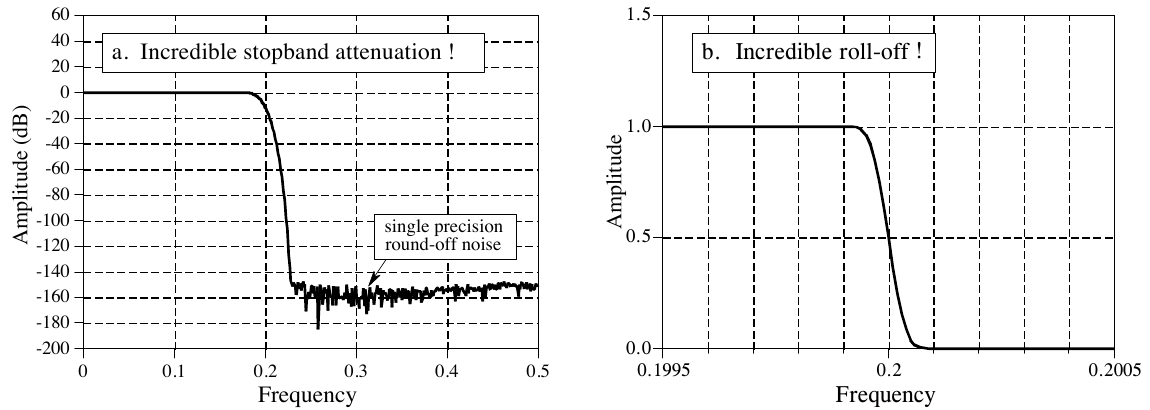
\includegraphics[width=0.958\linewidth,height=0.8\textheight,keepaspectratio]{assets/ch16/fig16-07.png}
\caption*{\textbf{图 16-7　加窗 sinc 滤波器惊人的性能。} (a)
是一个阻带衰减增强的加窗 sinc 滤波器的频率响应，这是把加窗 sinc
滤波器核与自身卷积得到的。(b) 是一个 32,001 点加窗 sinc
滤波器极快的滚降。 （a. Incredible stopband attenuation ! =
惊人的阻带衰减！b. Incredible roll-off ! = 惊人的滚降！single precision
round-off noise = 单精度舍入噪声。Amplitude = 幅度，Amplitude (dB) =
幅度（分贝），Frequency = 频率。）}
\end{figure}

图 16-7b 是加窗 sinc 惊人性能的另一个例子：一个滤波器核有 32,001
个点的低通滤波器。频率响应和预期的一样，滚降宽度是采样率的
0.000125。这个滤波器有多好？试着做一个模拟电子滤波器：让直流到 1000
赫兹的信号通过、变化小于 0.02\%，同时挡住 1001
赫兹以上的所有频率、残留小于
0.02\%。那才叫滤波器！如果你真想被震撼一下，记住图 16-7
中的两个滤波器都用的是单精度。用双精度还能把这些性能指标再扩展一百万倍。

加窗 sinc
滤波器最大的局限是执行时间：如果滤波器核点数很多，又用标准卷积，执行时间可能长得无法接受。第
18 章会介绍这种滤波器的一种高速算法（FFT 卷积）。递归滤波器（recursive
filter，第 19 章）也能提供良好的频率分离，是加窗 sinc
滤波器的一个合理替代。

加窗 sinc
是分离频率的最优滤波器核吗？不是，更复杂的技术得到的滤波器核可以更好。但要当心！在一头扎进这个非常数学化的领域之前，你应该想清楚自己到底想得到什么。加窗
sinc
能提供你可能需要的任何性能水平。高级滤波器设计方法能提供的，也许只是在给定性能下稍短一点的滤波器核，进而也许稍快一点的执行速度。要有心理准备：你付出的努力可能换不来多少回报。
